\chapter{Design des Artefakts}

In diesem Kapitel wird die Entwicklung der HoloLens Planner App zur Unterstützung von Fliesenlegers, welche für die Microsoft HoloLens entwickelt wird, beschrieben. Zum Entwickeln wurde Unity verwendet. Das Hololens Toolkit stellte benötigte Funktionalitäten zur Verfügung, welche beim Entwickeln für die Microsoft HoloLens essentiell sind.
Es wird nach der Methode für gestaltungsorientierte Forschung von Peffers (siehe Sektion \ref{sec:gestForsch}) vorgegangen. Die Probleme von Handwerkern, genauer Fliesenlegern, werden herausgearbeitet. Daraus werden Ziele für die zu entwickelnde Applikation abgeleitet. Diese Anwendung wird anschließend in einem iterativen Prozess über fünf Phasen entwickelt. Abschließend werden die Ergebnisse kommuniziert.

\section{Problemidentifikation und Motivation}

Aus der Ethnographie geht hervor, dass beim Verlegen der Fliesen Zeit verloren geht. Der Handwerker muss dabei jedes mal seinen Arbeitsfluss unterbrechen und im Raum nachmessen, um die Orientierungslinie korrekt anzuzeichnen. Dies macht er mit einer Schlagschnur, was jedoch schwierig wird, wenn er allein arbeitet. Müsste es diese Linie nicht anzeichnen, könnte er, unterstützt durch einen weiteren Arbeiter, der ihm Fliesen reicht, den gesamten Boden am Stück verlegen. Diese Linie ist jedoch essentiell wichtig, damit die Fliesen beim Verlegen nicht schief werden.

Laut Fokusgruppe und Ethnographie wäre ein Werkzeug, um den Raum zu erfassen und so die Planung zu vereinfachen, hilfreich. Die Wandlängen, Winkel und Unebenheiten zu messen nimmt einiges an Zeit in Anspruch. Schreibt der Handwerker sich dies nicht auf, hat er die Maße nur für den nächsten Arbeitsschritt im Kopf und muss das Vermessen oft wiederholen. Das kostet den Handwerker viel Zeit, wie in der Fokusgruppe hervorgehoben. Fliesenleger müssen bei diesem Schritt auch an den Fliesenverschnitt denken. Sie wollen Fliesen, die auf weniger als 2cm zurechgeschnitten werden müssen unbedingt vermeiden. Eine visuelle Darstellung des Raumes wäre dabei förderlich. 

Ein weiteres Problem ist die Abstimmung mit anderen Handwerkern. Erledigte oder geplante Aufgaben werden oft per Telefon kommuniziert, wodurch viel Misskommunikation und Fehler entstehen können. Besonders in dem Fall, dass ein Handwerker das Kundengespräch leitet und seine Kollegen anschließend über die Pläne informiert, wie aus der Fokusgruppe hervorgeht. Der Handwerker aus der Ethnographie merkte an, dass der Vertrag mit dem Kunden aus selbem Grund häufig nicht richtig spezifiziert ist und er so falsch umgesetzt wird.

Das größte Problem, bei welchem sich die Handwerker der Fokusgruppe, sowie der Ethnographie einig waren, ist die mangelnde Vorstellungskraft der Kunden. Der Handwerker kann sich das Ergebnis seiner Arbeit im Rohbau bereits vorstellen, da er die Erfahrung hat, der Kunde jedoch nicht und mit Worten ist so etwas schwer zu beschreiben, wie in der Ethnographie erläutert wird. Dadurch ist es für den Handwerker auch schwer dem Kunden zu zeigen, warum er etwas anders machen würde als dieser sich vorstellt. Oft reden Handwerker und Kunde bei diesen Gesprächen aneinander vorbei. Einen technischen Bauplan versteht der Laie auch nicht und Skizzen helfen nur mäßig. Dabei kommt es oft zu Ambiguität in den Kundengesprächen.

\section{Ziele der Lösung}

Mit der Lösung wird angestrebt, die Pläne des Fliesenlegers zu visualisieren und ihn bei der Arbeit zu unterstützen. \\
Lassen sich die Pläne des Handwerkers direkt betrachten, ist es einfacher für beide Parteien Änderungen vorzuschlagen, zu positionieren und zu beschreiben. Am besten sollte dies direkt im Rohbau möglich sein. Durch die Visualisierung können Pläne auch zwischen Handwerkern deutlicher kommuniziert werden. \\
Zur Unterstützung beim Fliesenlegen soll das erstellte Programm den Raum vermessen können und dies auch automatisch dokumentieren, sodass die Informationen jederzeit eingesehen werden können. Außerdem soll es möglich sein zu vermeiden, dass die Fliesen beim verlegen schief werden. Es wird also eine virtuelle Orientierungslinie oder Ähnliches benötigt.

\section{Entwicklung des Artefakts}

Die folgenden Abschnitte beschreiben die einzelnen Schritte der Entwicklung der App. Mit kleinen Evaluationsrunden wurde diese über fünf Iterationen verbessert und benutzerfreundlicher gemacht.

\subsection{Phase 1}

\subsubsection{Gestaltung und Entwicklung}

Anfangs wurde der Fokus auf die Funktionalität zum Boden bestimmen und Fliesen verlegen gelegt. Unterstützung bei der Arbeit des Fliesenlegers wird ab Phase 4 hinzugefügt. 

Zur Navigation durch die Funktionen der Applikation wird ein Menü designed mit den Schaltflächen \enquote{Bodenfläche abstecken}, sowie \enquote{Fliesen verlegen}. Das dient dazu, navigieren zu können, falls die Bodenfläche angepasster werden soll.

\begin{figure}[h]
	\begin{center}
		\noindent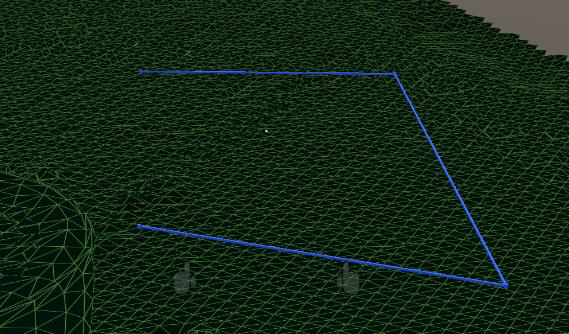
\includegraphics[scale=0.7]{Resources/Artefakt/bodenAbstecken.png}
		\label{abstecken}
		\caption{Abstecken des Bodens}	
	\end{center}
\end{figure}

Die Microsoft HoloLens besitzt \textbf{spatial mapping}, was sie dazu nutzt, um sich ein internes Bild ihrer Umgebung zu erzeugen. Diese Funktion unterscheidet allerdings nicht zwischen \enquote{Wand}, \enquote{Boden} oder \enquote{Decke}. Daher muss der Boden händisch festgelegt werden. Dazu platziert der Nutzer in den Ecken des Raumes kleine Punkte, welche automatisch durch Linien miteinander verbunden werden (siehe Abbildung \ref{abstecken}). Durch \enquote{Klicken \& Halten} wird daraus die Bodenfläche erstellt, auf der anschließend die Fliesen verlegt werden sollen.

\begin{figure}[h]
	\begin{center}
		\noindent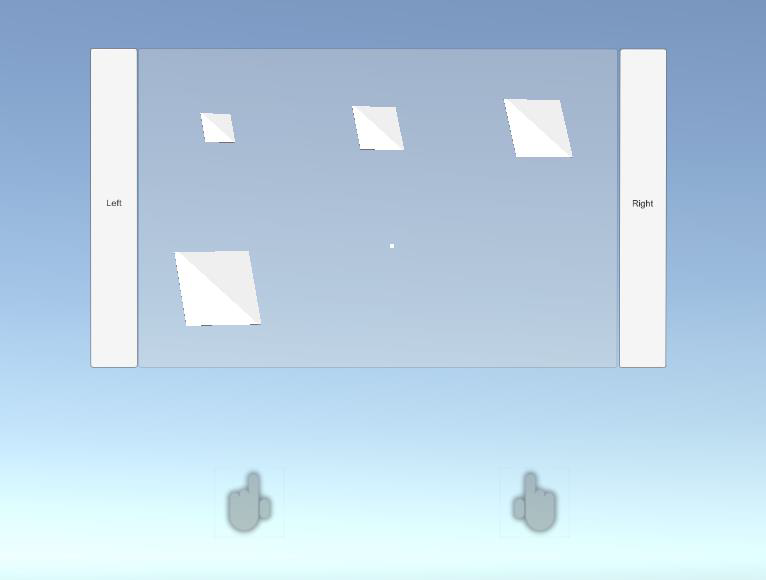
\includegraphics[scale=0.50]{Resources/Artefakt/auswahlAlt.png}
		\label{fliesenwahlAlt}
		\caption{Altes Menü zur Fliesenauswahl}	
	\end{center}
\end{figure}

\begin{figure}[h]
	\begin{center}
		\noindent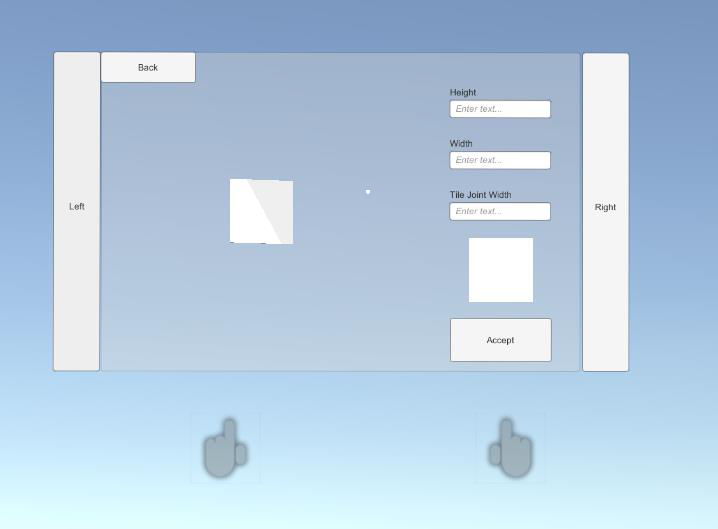
\includegraphics[scale=0.55]{Resources/Artefakt/detailAlt.png}
		\label{fliesendetailAlt}
		\caption{Altes Menü für Detailansicht}	
	\end{center}
\end{figure}

Das Fliesenmenü präsentiert in einem 3x2 Grid eine Auswahl an verschiedenen Fliesen (siehe Abbildung \ref{fliesenwahlAlt}). Wählt der Nutzer eine davon, öffnet sich eine Detailansicht der Fliese, welche alle Informationen dazu in Textfeldern anzeigt (siehe Abbildung \ref{fliesendetailAlt}). Diese beinhalten Breite, Länge, Fugenweite und die Textur der Fliese. In dieser Ansicht ist es auch möglich die Fliese zu bearbeiten. Zusätzlich können neue Fliesen angelegt und in den Katalog eingefügt werden.

\begin{figure}[h]
	\begin{center}
		\noindent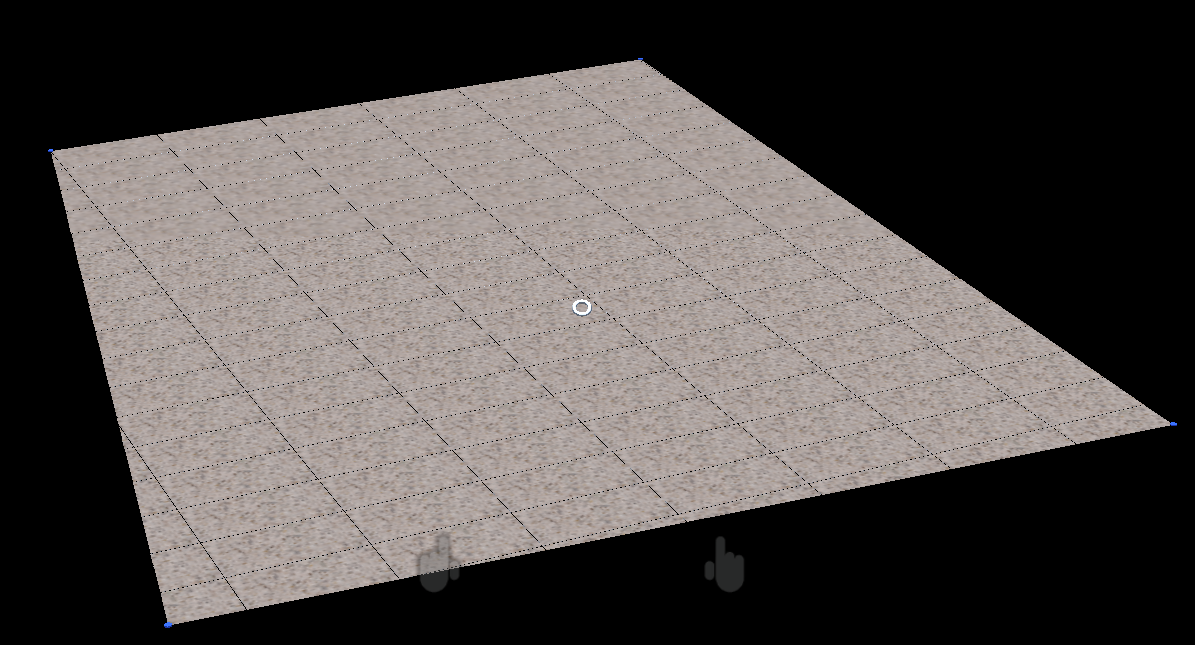
\includegraphics[scale=0.4]{Resources/Artefakt/bodenVerlegt.png}
		\label{bodenVerl}
		\caption{Virtuell verlegte Fliesen}	
	\end{center}
\end{figure}

Wurde die Bearbeitung abgeschlossen, müssen die Fliesen verlegt werden. Dabei erschien es am besten für einen Prototypen, die Fliesen entlang einer Kannte des Bodens zu verlegen. Dafür wählt der Nutzer einen Eckpunkt der Fläche als Startpunkt und einen weiteren als Richtungspunkt. Sind diese gewählt, verlegt die Applikation die Fliesen virtuell (siehe Abbildung \ref{bodenVerl}).

\subsubsection{Demonstration des Artefakts}

Zur Demonstration des ersten Prototypen wurden zwei Studenten der Fakultät Informatik der Technischen Universität München gewählt. Sie sollten die Applikation in einem teilweise möblierten Raum testen. Vor dem Test wurde nur festgelegt, was das Ergebnis sein sollte. Währenddessen wurde versucht keine Anweisungen gegeben.

\subsubsection{Evaluation}

Das Szenario war für die Studenten, obwohl sie technisch aversiert sind, schwer ohne Anweisungen durchführbar. Es vielen dabei einige Verbesserungsmöglichkeiten auf. 

Beim Abstecken der Bodenfläche hat der Nutzer keine Möglichkeit Fehler zu beheben. Wurde ein Punkt, evtl. durch einen unbeabsichtigten Klick, falsch positioniert, gab es keine Option, um das rückgängig zu machen. \\
Die Daten in den Textfeldern waren sehr klein geschrieben und daher schwer zu lesen. Noch dazu bemängelten die Probanden, dass es nicht elegant wirke. \\
Aus der Detailansicht zum Bearbeiten der Fliesen konnte man nicht auf die Fliesenauswahl zurücknavigieren, was die Probanden auch bemängelten.

\subsection{Phase 2}

\subsubsection{Gestaltung und Entwicklung}

Um Fehler beim Abstecken der Bodenfläche beheben zu können, wurde eine Funktion eingebaut, mit der der zuletzt gesetzte Punkt durch Anklicken gelöscht werden kann. 

\begin{figure}[h]
	\begin{center}
		\noindent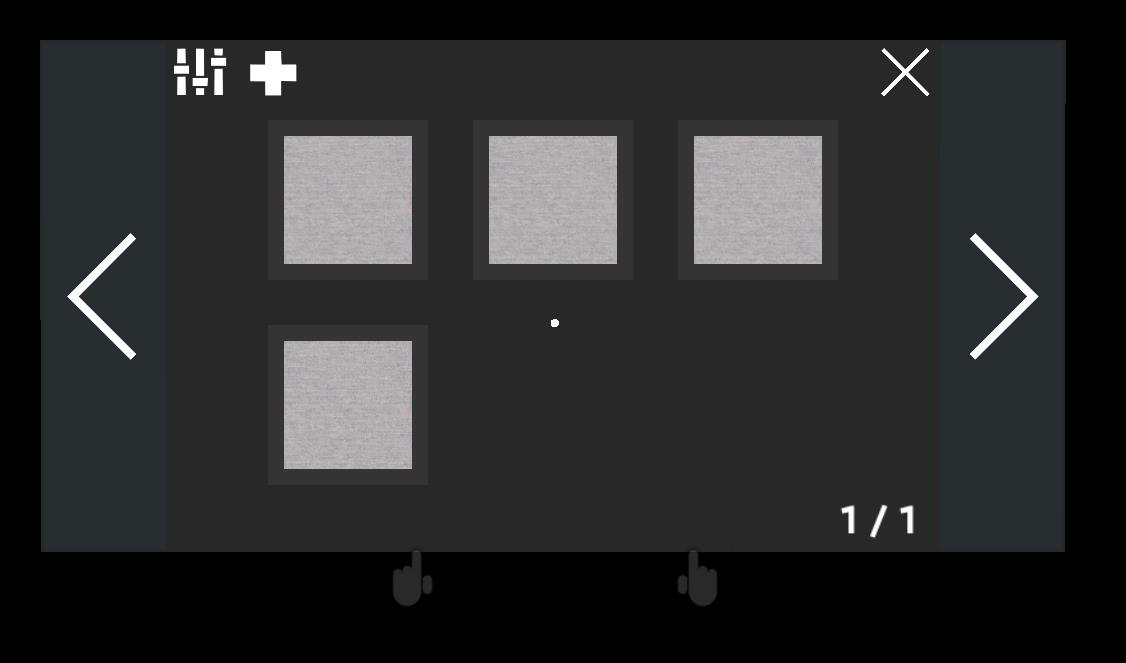
\includegraphics[scale=0.4]{Resources/Artefakt/auswahl.png}
		\label{auswahl}
		\caption{Neues Design der Fliesenauswahl}	
	\end{center}
\end{figure}

Das Design der Fliesen Detailansicht wurde umgebaut, um es mit natürlichen, selbsterklärenden Schaltflächen intuitiver zu machen und um Textboxen zu eliminieren. Dabei wurde auch das gesamte Design der App dunkler gemacht (siehe Abbildung \ref{auswahl}). Zusätzlich wurde eine Einstellungsmöglichkeit für die Tiefe der Fliesen eingefügt (siehe Abbildung \ref{detail}).

\begin{figure}[h]
	\begin{center}
		\noindent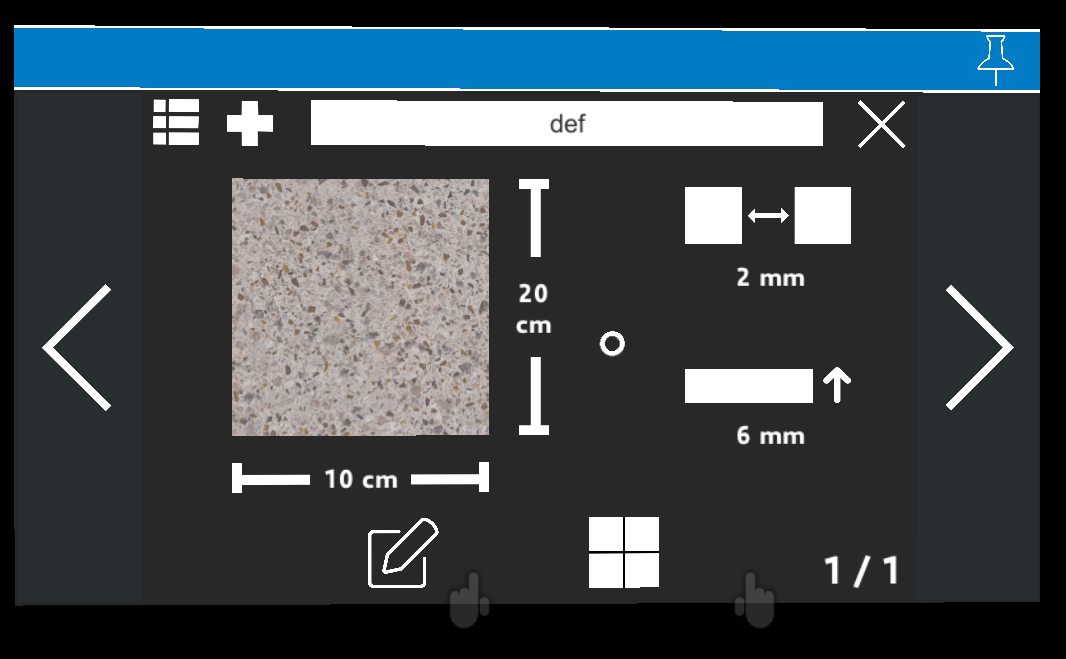
\includegraphics[scale=0.4]{Resources/Artefakt/detail.png}
		\label{detail}
		\caption{Neues Design der Detailansicht}	
	\end{center}
\end{figure}

Für den Wechsel zwischen Fliesenauswahl Ansicht und Fliesen Detailansicht wurde ein entsprechender Button eingefügt.

\subsubsection{Demonstration des Artefakts}

Es wurden erneut zwei Studenten der Fakultät für Informatik der TU München ausgewählt, um die Applikation zu testen. Dafür wurde der selbe teilweise möblierte Raum genutzt. Es wurde geplant während des Tests nur Anweisungen zu geben, wenn der Proband nicht weiter kommt.

\subsubsection{Evaluation}

Beide Probanden fanden das Erzeugen der Bodenfläche durch \enquote{Klicken \& Halten} wenig intuitiv. Außerdem viel auf, wenn man eine neue Bodenfläche erstellen möchte, bleibt die alte weiter bestehen. Das sollte nicht passieren. \\
In der neuen Detailansicht war nicht ersichtlich welcher Button zum Verlegen der Fliesen führt, da dafür nun Symbole, statt Worte als Beschreibung verwendet wurden. \\
Auch das Verlegen der Fliesen wurde von einem Probanden als nicht intuitiv beschrieben.

\subsection{Phase 3}

\subsubsection{Gestaltung und Entwicklung}

Es wurde Tutorialtext eingefügt, welcher das Abstecken des Bodens beschreibt. Dieser geht auch darauf ein, dass man zum erstellen \enquote{Klicken \& Halten} muss (siehe Abbildung \ref{tutBoden}). \\
Das Verlegen der Fliesen wird jetzt auch mit Tutorialtext beschreiben (siehe Abbildung \ref{tutFliesen}). \\
Diese Tutorialtexte sind nicht irgendwo im Blickfeld fixiert, sondern folgen dem Gaze. Damit der Text nicht beim Arbeiten am Boden stört, wurde die Option eingefügt, ihn im Raum zu fixieren. Ein weißer Pfeil deutet dann auf diesen, damit man ihn wiederfindet. Die Information die UI so zu erstellen, stammt auf diesem Video: \url{https://www.youtube.com/watch?v=sX6yKHmN1qM}.

\begin{figure}[h]
	\begin{center}
		\noindent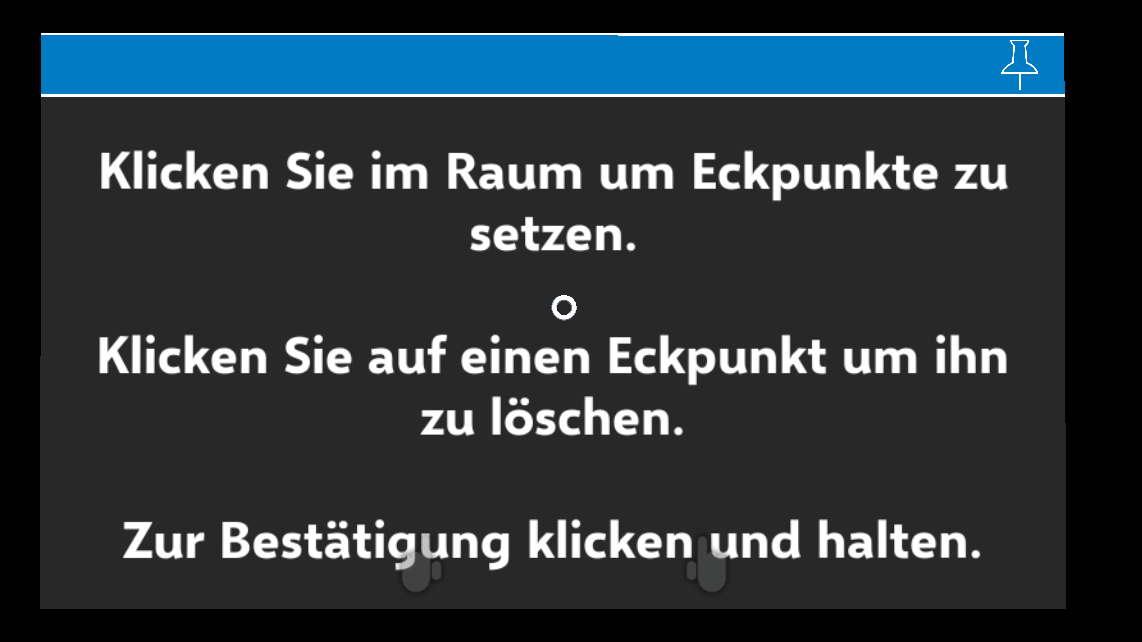
\includegraphics[scale=0.4]{Resources/Artefakt/bodenText.png}
		\label{tutBoden}
		\caption{Tutorialtext zum Abstecken des Bodens}	
	\end{center}
\end{figure}

\begin{figure}[h]
	\begin{center}
		\noindent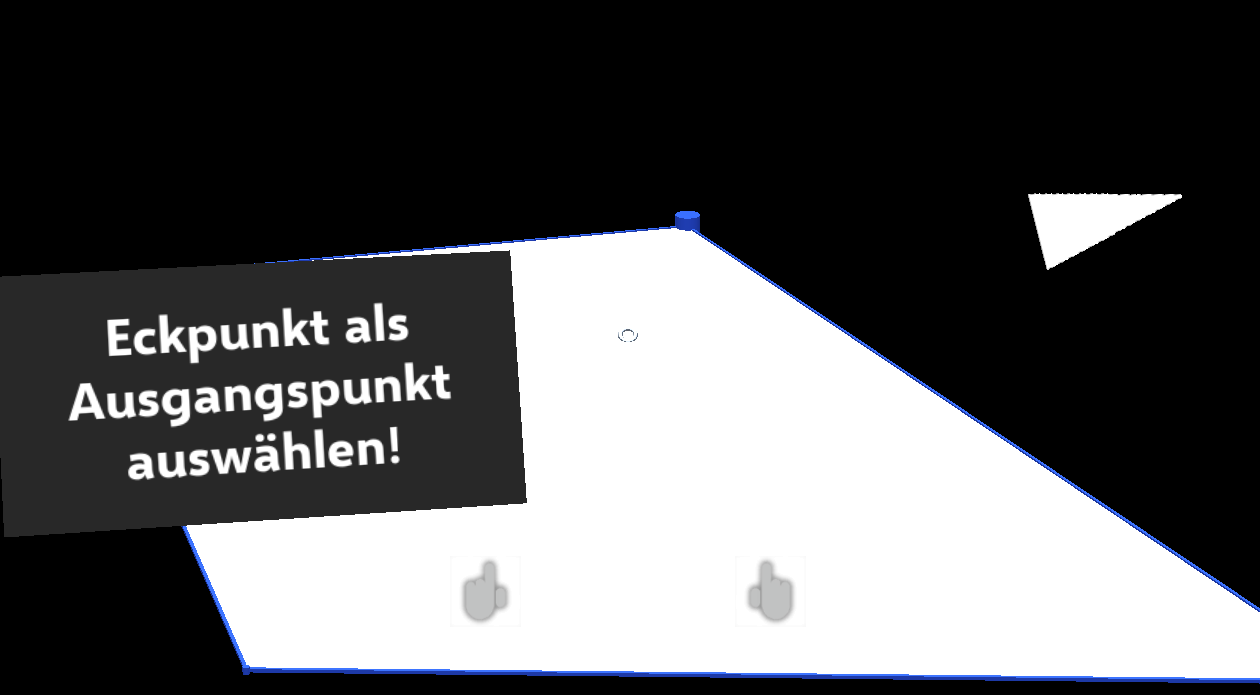
\includegraphics[scale=0.4]{Resources/Artefakt/verlegenText.png}
		\label{tutFliesen}
		\caption{Tutorialtext zum Verlegen der Fliesen}	
	\end{center}
\end{figure}

Falls bereits ein Boden erstellt wurde, dieser jedoch nicht genau genug ist und der Nutzer daher einen neuen erstellt, wird der alte Boden automatisch gelöscht.

Damit die Funktionalität der Symbole der Buttons im Fliesen Detailmenü ersichtlicher ist, wurde ein Beschreibungstext eingefügt, welcher erscheint, wenn der Nutzer den Gaze darauf richtet.

\subsubsection{Demonstration des Artefakts}

Dieses mal wurde die Applikation erneut mit zwei Studenten der TU München, als auch mit einem Wissenschaftlichen Mitarbeiter. Dafür wurde der selbe Raum wie bei den ersten Tests verwendet. Anweisungen wurden nur wenn nötig gegeben.

\subsubsection{Evaluation}

Beim Abstecken des Bodens können teilweise Punkte nicht gesetzt werden. Das behindert die Funktionalität und frustriert den Nutzer. Der wissenschaftliche Mitarbeiter merkte an, dass es für die Genauigkeit der Bodenfläche gut wäre, wenn man die Eckpunkte nachträglich verschieben und so präziser in den Ecken positionieren könnte. \\
Das Menü folgt dem Gaze un behindert so teilweise das Verlegen der Fliesen.

\subsection{Phase 4}

\subsubsection{Gestaltung und Entwicklung}

Die Eckpunkte sind nur auf \enquote{gemappetem} Areal setzbar, also Boden, den die HoloLens schon selbst gescanned und realisiert hat. Um das zu verdeutlichen wird das spatial mapping nun mit einem grünen Gitter angezeigt (siehe Abbildung \ref{abstecken}). So erkennt der Nutzer genau, welche Teile des Raums bereits gemapped sind und welche noch nicht.

\begin{figure}[h]
	\begin{center}
		\noindent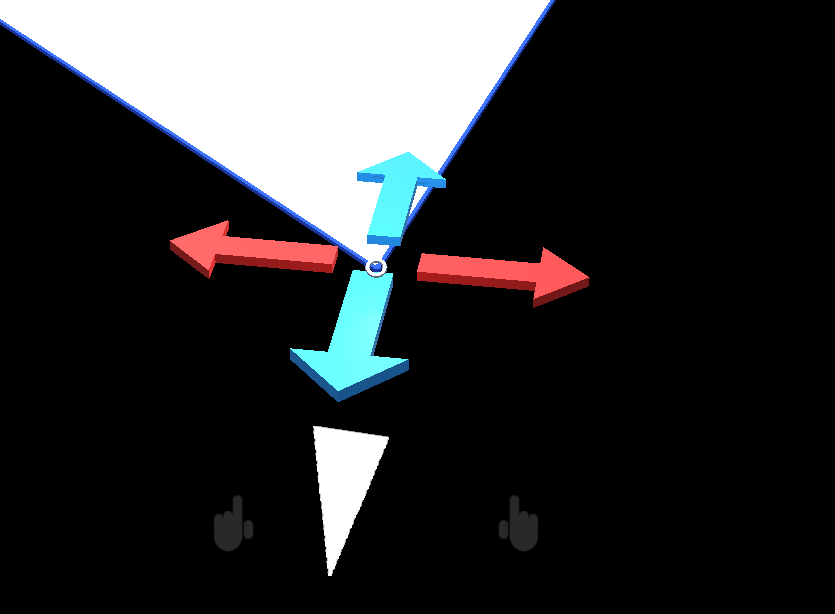
\includegraphics[scale=0.5]{Resources/Artefakt/punktVersch.png}
		\label{pfeile}
		\caption{Pfeile zum Verschieben der Eckpunkte}	
	\end{center}
\end{figure}

\begin{figure}[h]
	\begin{center}
		\noindent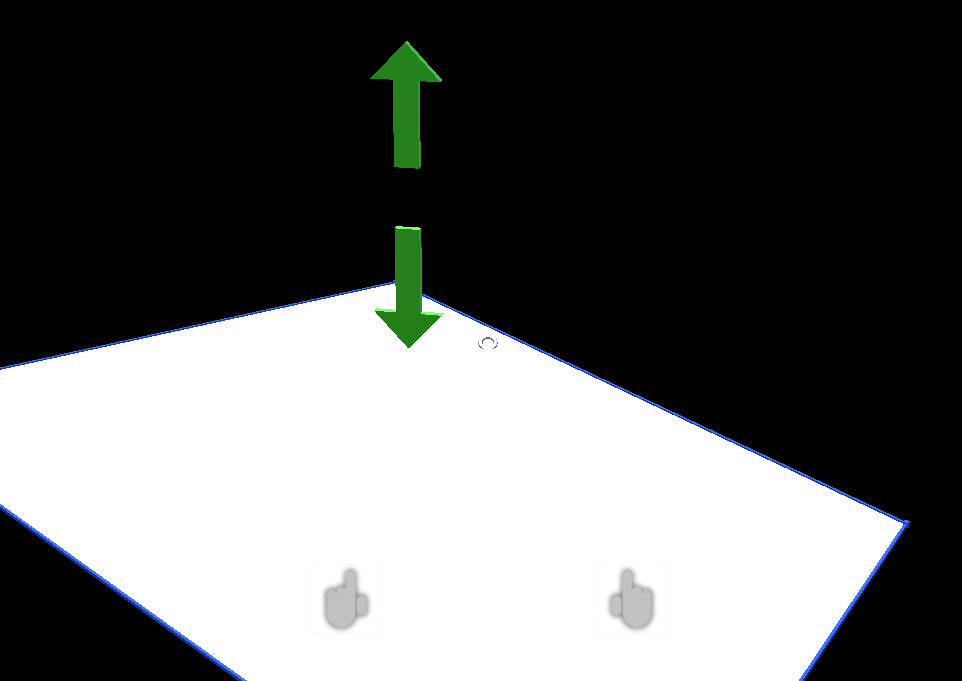
\includegraphics[scale=0.4]{Resources/Artefakt/bodenUpDown.png}
		\label{pfeileBoden}
		\caption{Pfeile zum verschieben der Bodenfläche}	
	\end{center}
\end{figure}

Sobald die Bodenfläche erstellt ist, kann der Nutzer die einzelnen Eckpunkte nun verschieben. Wählt er einen davon aus erscheinen rundherum Pfeile (siehe Abbildung \ref{pfeile}). Mit diesen kann er den Punkt in 0,5cm Schritten in beliebige Richtungen bewegen und die Eckpunkte so präziser setzen. Zusätzlich wurde vorbeugend die Funktionalität eingebaut, mit Pfeilen die gesamte Fläche hoch oder runter zu bewegen (siehe Abbildung \ref{pfeileBoden}). Das soll helfen, falls Teile der Bodenfläche im \enquote{realen Boden verschwinden}.

Damit das Menü beim Arbeiten nicht mehr stört, wurde eine \textit{pin-Funktion} implementiert. Mit Klick auf die Schaltfläche wird das Menü an eine Stelle im Raum gepinnt und kann so auch wieder gelöst werden (siehe Abbildung \ref{menue}). Ein weißer Pfeil leitet den Nutzer zum Menü zurück, falls er es verlieren sollte.

\begin{figure}[h]
	\begin{center}
		\noindent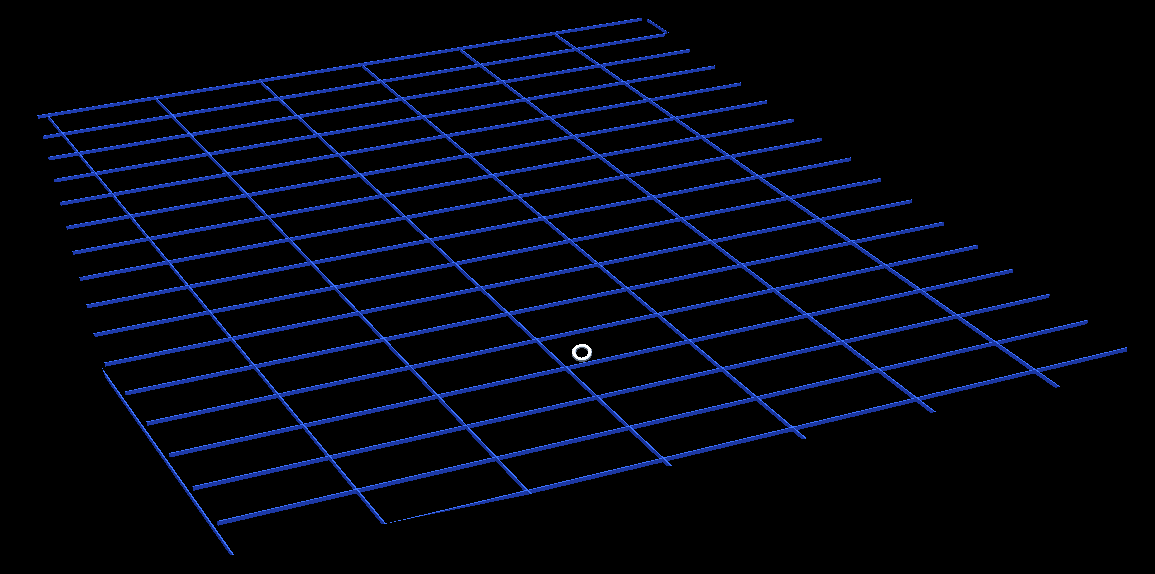
\includegraphics[scale=0.4]{Resources/Artefakt/verlegeassistent.png}
		\label{assistent}
		\caption{Assistent zum Fliesenverlegen}	
	\end{center}
\end{figure}

\begin{figure}[h]
	\begin{center}
		\noindent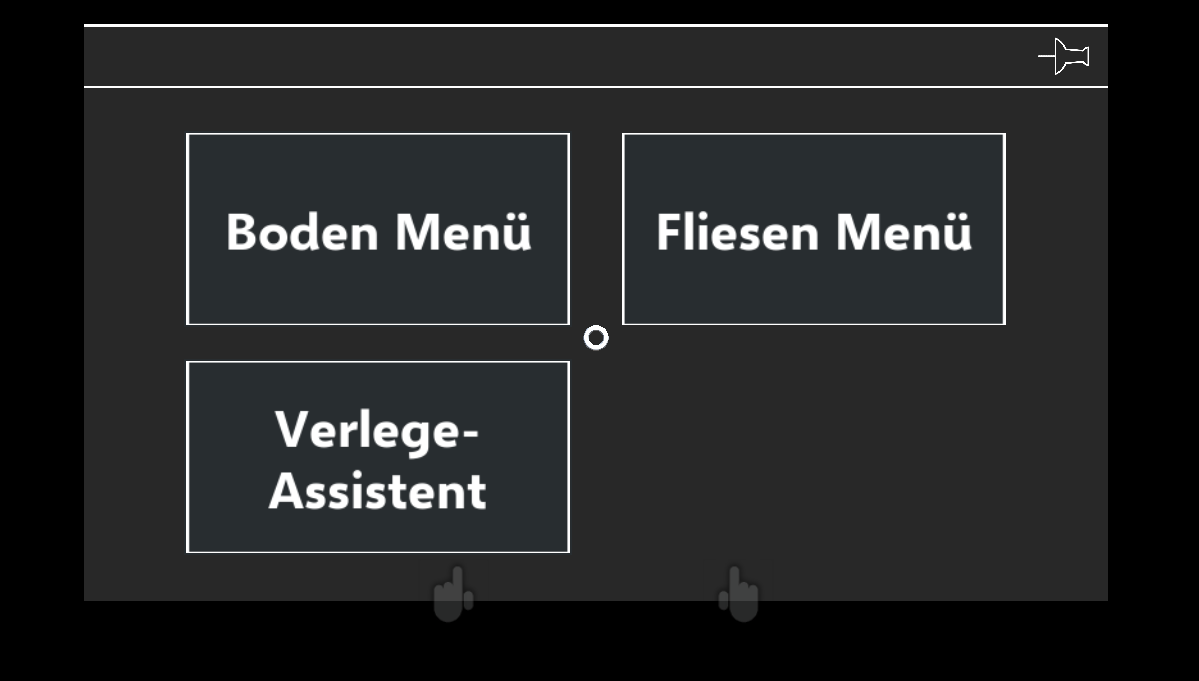
\includegraphics[scale=0.4]{Resources/Artefakt/menue.png}
		\label{menue}
		\caption{Startmenü mit Pin-Button oben rechts}	
	\end{center}
\end{figure}

In dieser Iteration wurde auch ein Assistent zum Fliesenverlegen implementiert. Durch einen neuen Button im Menü kann dieser aktiviert werden. Das ist allerdings erst nach dem Verlegen der Fliesen möglich. Er lässt die Fliesen verschwinden und zeigt nur noch deren Fugen in blau an (siehe Abbildung \ref{assistent}). So stellt er dem Handwerker ein Gitter, in welches er nur noch die echten Fliesen einzulegen braucht.

\subsubsection{Demonstration des Artefakts}

Diese Demonstration wurde mit zwei Wissenschaftlichen Mitarbeitern der Fakultät für Wirtschaftsinformatik der TU München durchgeführt. Sie fand im selben Raum statt. Diesmal wurde den Probanden ein Szenario vorgegeben. Sie sollten eine festgelegte Fläche abstecken, darauf Fliesen verlegen und alle Funktionen des HoloLens Planners einmal testen.

\subsubsection{Evaluation}

Die Tutorialtexte und alle anderen waren bis jetzt auf Englisch. Da die App zum Abschluss noch mit deutschen Handwerkern getestet werden sollte, wäre es von Vorteil diese auf Deutsch zu übersetzen. \\
Die Pfeile zum Verschieben der Punkte wurden, laut der Probanden, zu groß angezeigt. Dadurch verliert man beim Bedienen den Überblick.

\subsection{Phase 5}

\subsubsection{Gestaltung und Entwicklung}

Die Pfeile für das Verschieben der Punkte wurden verkleinert. Alle Texte der Applikation wurden ins Deutsche übersetzt.

\begin{figure}[h]
	\begin{center}
		\noindent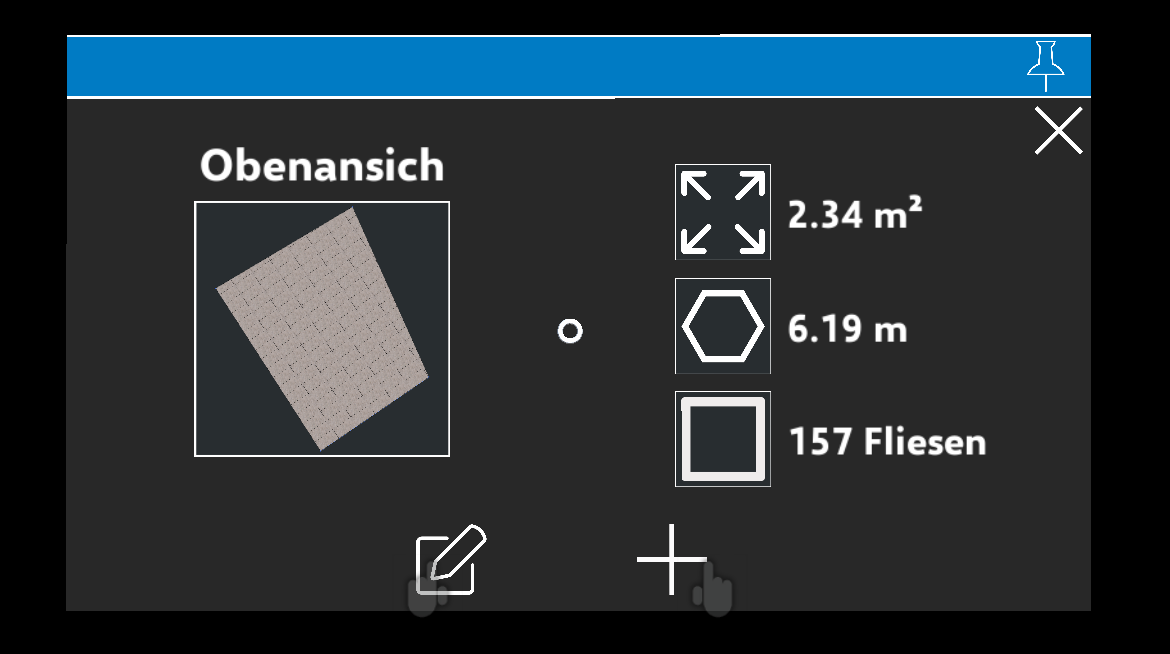
\includegraphics[scale=0.4]{Resources/Artefakt/datenBoden.png}
		\label{daten}
		\caption{Daten zum verlegten Boden}	
	\end{center}
\end{figure}

Zu guter Letzt wurde die Funktionalität zum Anzeigen wichtiger Metriken umgesetzt. Im Bodenmenü kann der Fliesenleger nun einsehen, wie groß die Fläche in Quadratmetern ist und wie viel Umfang sie hat (siehe Abbildung \ref{daten}). Zusätzlich, vorausgesetzt der Handwerker hat virtuell bereits die Fliesen verlegt, zeigt diese Ansicht ihm die Anzahl der benötigten Fliesen an.

\subsubsection{Demonstration des Artefakts und Evaluation}

Die Finale Demonstration und Evaluation der HoloLens Planner Applikation mit allen Funktionalitäten wird mit Handwerkern durchgeführt. Die Durchführung und Ergebnisse davon werden im nächsten Kapitel kommuniziert. 